

\section{Laning and Zierler at MIT}
\label{sec:laning-zierler}

Of the early compiler efforts, Laning and Zierler's team is perhaps the most overshadowed.
Their contemporaries were very impressed by their work, and they inspired a number
of innovations at Remington Rand and IBM.
Backus described the pseudocode compilers of the time (such as the A-2)
as merely providing an instruction set
slightly different from the machine's actual code, but not providing any real abstraction;
writing the pseudocode still tedious and unproductive.
Laning and Zierler's work was different.

John Backus was hugely supportive of their work, though he was not directly invluenced by it
prior to starting work on \GLS{ftn}.
In Backus's 1980 paper on the programming landscape of the 1950s
\citetitlecite{Backus_1980_Programming_in_America_in_1950s}, he recalls:

\begin{quotation}
	Very early in the 1950s, J. Halcombe Laning, Jr., recognized that
	programming using algebraic expressions would be an important improvement.
	As a result of that insight he and Neal Zierler had the first
	algebraic compiler running on WHIRLWIND at MIT in January 1954.
	(A private communication from the Charles Stark Draper Laboratory indicates
	that they had demonstrated algebraic compiling sometime in 1952!) The priesthood
	ignored Laning's insight for a long time. A 1954 article by Charles W. Adams
	and Laning (presented by Adams at the ONR symposium) devotes less than
	3 out of 28 pages to Laning's algebraic system; the rest are devoted to other
	MIT systems. The complete description of the system's method of operation
	as given there is the following
\end{quotation}

In this quote, the \textit{priesthood} Backus is referring to is the group of programmers
who rejected the idea that programming should or could be done in a higher level language,
and that programming in machine code is an art that would need to be preserved.
On his own side of the argument, Backus found Laning and Zierler's work on compiling
algebraic expressions into programs to be more accessible and efficient.
Grace Hopper was on this side of the argument as well.
See Section \ref{sec:backus_priesthood} for more details about this debate.

Donald Knuth and Trabb Pardo also recall the importance of their work in
the development of programming languages and compilers
in \citetitlecite{Knuth_TrabbPardo_1976_Early_Development}:

\begin{quotation}
	In retrospect, the biggest event of the 1954 symposium on automatic
	programming was the announcement of a system that J. Halcombe Laning, Jr. and Niel Zierler
	had recently implemented for the Whirlwind computer at M.I.T.  However, the
	significance of that announcement is not especially evident from the published
	proceedings [NA 524-], 97\% of which are devoted to enthusiastic description s
	of assemblers, interpreters, and 1954-style "compilers".
\end{quotation}

Clearly, their work was influential.
The compiler system they described is often referred to as simply
\textit{Laning and Zierler's algebraic compiler}
because they never gave it a name.
They described its use in their paper \citetitlecite{laning_zierler_algebraic_compiler_manual_1954},
which describes problems that Backus and Hopper were also facing, such as syntactic ambiguities,
the likes of which would not be worked out until Alfred Aho's work at Bell Labs
\ref{sec:software-unix-regex}.

Their user manual gives the following example of an iterative algorithm for
calculating the power series of $cosine x$:

\begin{lstlisting}[frame=single]
    x = 0,
1   y = 10,
    z = 1,
2   z = 1 - z x^2/y (y - 1),
    y = y - 2,
    e = 1 - У,
    CP 2,
    PRINT x, Z.
    x = x + O.l,
    a = x - 1.05,
    CP 1,
    STOP
\end{lstlisting}

While this might seem trivial today, it was a significant deviation from the
best-known methods for computing at the time. To write a program with their algebraic
compiler, one needn't know anything about the machine the calculation was being performed on--the
programmer was free to consider only the mathematical results they were interested in.

They also provided a set of subroutines to their users which was, though quite inconvenient,
an early standard library.
In \cite[Section 11. Function Subroutines]{laning_zierler_algebraic_compiler_manual_1954},
they provide a table of supported subroutines:

\begin{quotation}
	It is clearly desirable to build into the computer subroutines
	that compute automatically certain frequently used functions. This
	process has been begun for our computer and at present the following
	functions are available:
	\\
	\begin{center}
		\begin{tabular}{|c|c|}
			\hline
			\underline{Designation} & \underline{Function} \\
			$F^1$                   & Square Root          \\
			$F^2$                   & sine                 \\
			$F^3$                   & cosine               \\
			$F^4$                   & tangent              \\
			$F^5$                   & $\sin^{-1}$          \\
			\hline
		\end{tabular}
	\end{center}

	The sine of x may be obtained by writing simply $F^{2}(x)$ and
	such an expression may be treated arithmetically in the same way
	as a variable in an equation.
\end{quotation}

Inconvenient as it would have been to keep track of the function of each function
by number rather than by name, Laning and Zierler were primarily concerned with
how readily a programmer could convert their mathematics into a useful program.
This higher level of abstraction set them apart from their peers and inspired
similar developments.

\begin{quotation}
	The first programming system to operate in the sense of a modern compiler was
	developed by J. H. Laning and N. Zierler for the Whirlwind computer at the
	Massachusetts Institute of Technology in the early 1950s. They described their
	system, which never had a name, in an elegant and terse manual entitled "A
	Program for Translation of Mathematical Equations for Whirlwind I,"
	distributed
	by MIT to about one-hundred locations in January 1954.26 It was, in John
	Backus's words, "an elegant concept elegantly realized." Unlike the UNIVAC
	compilers, this system worked much as modern compilers work; that is, it took
	as its input commands entered by a user, and generated as output fresh and
	novel machine code, which not only executed those commands but also kept track
	of storage locations, handled repetitive loops, and did other housekeeping
	chores. Laning and Zierler's "Algebraic System" took commands typed
	in familiar
	algebraic form and translated them into machine codes that Whirlwind could
	execute.27 (There was still some ambiguity as to the terminology: while Laning
	and Zierler used the word "translate" in the title of their manual, in the
	Abstract they call it an "interpretive program.")28
	\cite{new-history-of-modern-computing}
\end{quotation}

\begin{figure}[h!]
	\centering
	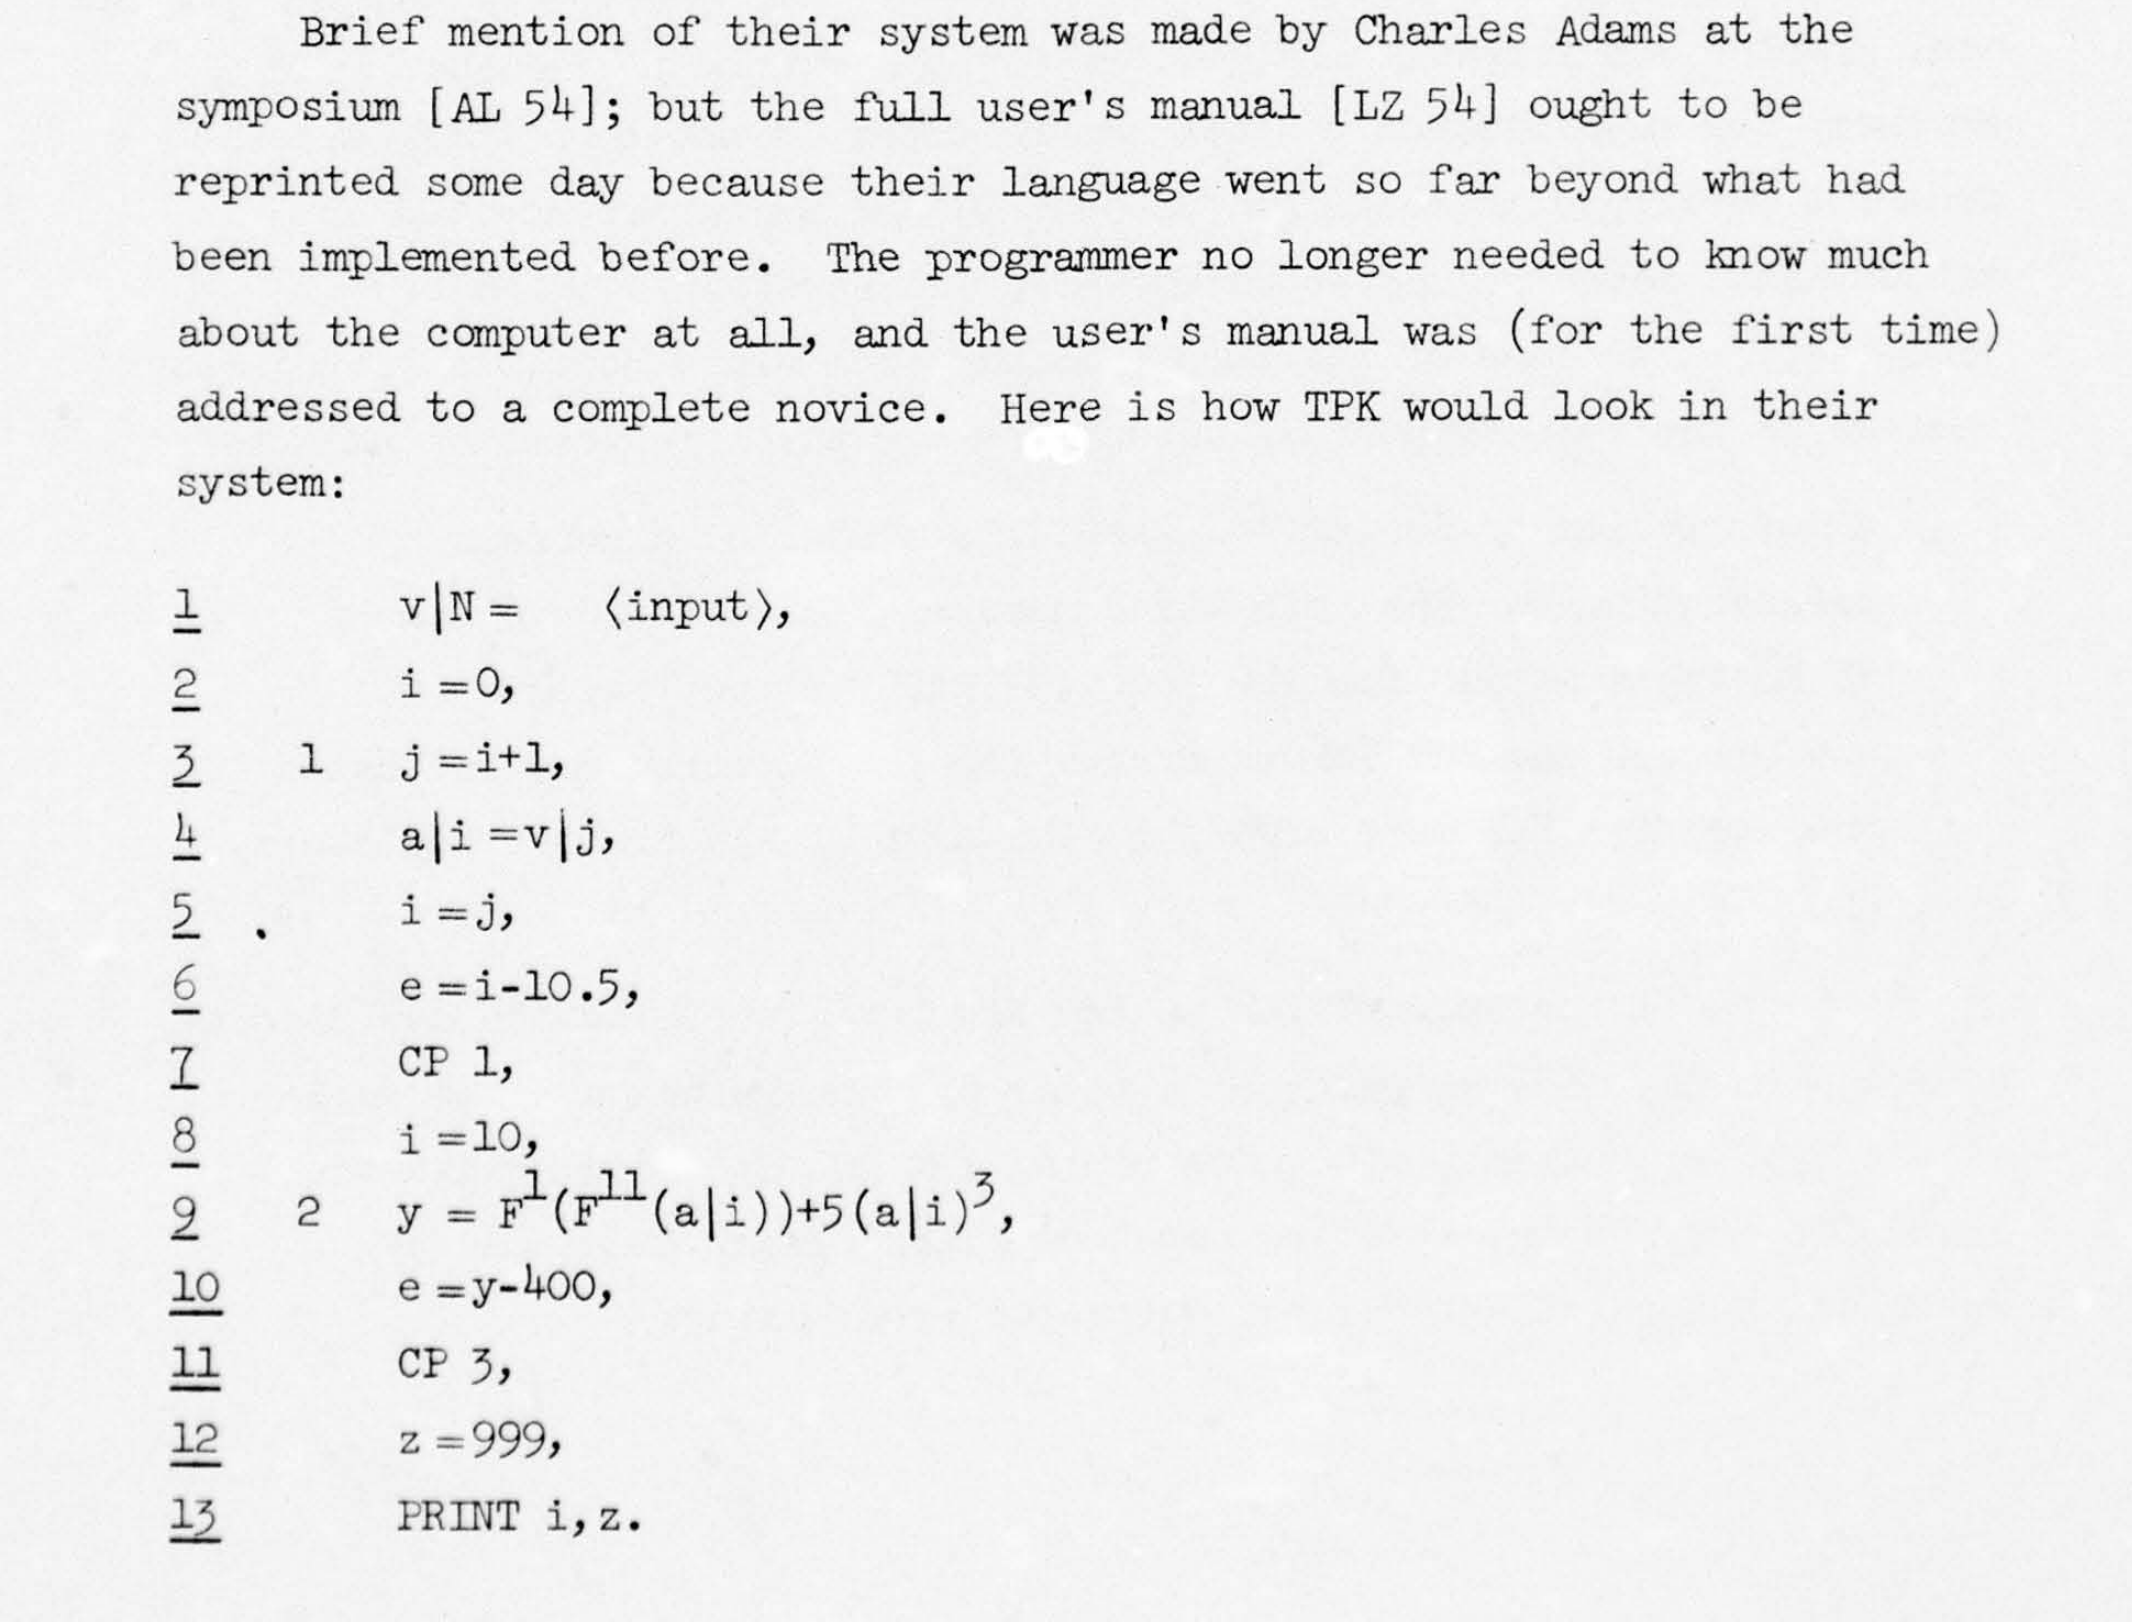
\includegraphics[width=0.5\linewidth]{resource/knuth_pardo_on_laning_zierlers_algebraic_compiler.png}
	\caption{Knuth and Pardo on Laning and Zierler's Algebraic Compiler}
	\label{fig:knuth-pardo-on-laning-zierler}
\end{figure}

\todo{Backus programming in the 50s has lots to say about this.}
\begin{quotation}
	Laning and Zierler's algebraic compiler served as evidence that prestigious
	institutions such as MIT were taking automatic programming
	seriously, prompting
	Backus to write Laning a letter shortly after the May symposium.
	In the letter,
	Backus informed Laning that his team at IBM was working on a
	similar compiler,
	but that they had not yet done any programming or even any
	detailed planning.12
	To help formulate the specifications for their proposed language, Backus
	requested a demonstration of the algebraic compiler, which he and Ziller
	received in the summer of 1954. Much to their dismay, the two
	experienced firsthand the efficiency dilemma of compiler-based
	language design. The MIT
	source code was commendable, but the compiler slowed down the Whirlwind
	computer by a factor of 10. Since computer time was so dear a
	commodity, Backus
	realized that only a compiler that maximized efficiency could
	hope to compete
	with human programmers. Despite this initial disappointment, Laning and
	Zierler's work inspired Backus to attempt to build a compiler that could
	translate a rich mathematical language into a sufficiently
	economical program
	at a relatively low cost.13
	\cite{grace_hopper_and_the_invention_of_the_information_age_2009}
\end{quotation}
